% Options for packages loaded elsewhere
\PassOptionsToPackage{unicode}{hyperref}
\PassOptionsToPackage{hyphens}{url}
\PassOptionsToPackage{dvipsnames,svgnames,x11names}{xcolor}
%
\documentclass[
  a4paper,
]{article}

\usepackage{amsmath,amssymb}
\usepackage{lmodern}
\usepackage{iftex}
\ifPDFTeX
  \usepackage[T1]{fontenc}
  \usepackage[utf8]{inputenc}
  \usepackage{textcomp} % provide euro and other symbols
\else % if luatex or xetex
  \usepackage{unicode-math}
  \defaultfontfeatures{Scale=MatchLowercase}
  \defaultfontfeatures[\rmfamily]{Ligatures=TeX,Scale=1}
  \setmonofont[]{Consolas}
\fi
% Use upquote if available, for straight quotes in verbatim environments
\IfFileExists{upquote.sty}{\usepackage{upquote}}{}
\IfFileExists{microtype.sty}{% use microtype if available
  \usepackage[]{microtype}
  \UseMicrotypeSet[protrusion]{basicmath} % disable protrusion for tt fonts
}{}
\makeatletter
\@ifundefined{KOMAClassName}{% if non-KOMA class
  \IfFileExists{parskip.sty}{%
    \usepackage{parskip}
  }{% else
    \setlength{\parindent}{0pt}
    \setlength{\parskip}{6pt plus 2pt minus 1pt}}
}{% if KOMA class
  \KOMAoptions{parskip=half}}
\makeatother
\usepackage{xcolor}
\usepackage[top=30mm,left=20mm,heightrounded]{geometry}
\setlength{\emergencystretch}{3em} % prevent overfull lines
\setcounter{secnumdepth}{5}
% Make \paragraph and \subparagraph free-standing
\ifx\paragraph\undefined\else
  \let\oldparagraph\paragraph
  \renewcommand{\paragraph}[1]{\oldparagraph{#1}\mbox{}}
\fi
\ifx\subparagraph\undefined\else
  \let\oldsubparagraph\subparagraph
  \renewcommand{\subparagraph}[1]{\oldsubparagraph{#1}\mbox{}}
\fi


\providecommand{\tightlist}{%
  \setlength{\itemsep}{0pt}\setlength{\parskip}{0pt}}\usepackage{longtable,booktabs,array}
\usepackage{calc} % for calculating minipage widths
% Correct order of tables after \paragraph or \subparagraph
\usepackage{etoolbox}
\makeatletter
\patchcmd\longtable{\par}{\if@noskipsec\mbox{}\fi\par}{}{}
\makeatother
% Allow footnotes in longtable head/foot
\IfFileExists{footnotehyper.sty}{\usepackage{footnotehyper}}{\usepackage{footnote}}
\makesavenoteenv{longtable}
\usepackage{graphicx}
\makeatletter
\def\maxwidth{\ifdim\Gin@nat@width>\linewidth\linewidth\else\Gin@nat@width\fi}
\def\maxheight{\ifdim\Gin@nat@height>\textheight\textheight\else\Gin@nat@height\fi}
\makeatother
% Scale images if necessary, so that they will not overflow the page
% margins by default, and it is still possible to overwrite the defaults
% using explicit options in \includegraphics[width, height, ...]{}
\setkeys{Gin}{width=\maxwidth,height=\maxheight,keepaspectratio}
% Set default figure placement to htbp
\makeatletter
\def\fps@figure{htbp}
\makeatother

\usepackage{ctex}    % CJK 包
\usepackage[backend=biber,style=gb7714-2015,gbnamefmt=lowercase]{biblatex}
\usepackage[dvipsnames]{xcolor}
\setCJKmainfont[AutoFakeBold = {2.25}]{宋体}
\setmainfont{Times New Roman} %英文字體調整
\usepackage{caption}
\DeclareCaptionLabelSeparator{bar}{ | }
\captionsetup[figure]{labelformat=simple, labelsep=bar,singlelinecheck=off, labelfont = bf}
\captionsetup[table]{labelformat=simple, labelsep=bar, labelfont = bf}
\makeatletter
\makeatother
\makeatletter
\makeatother
\makeatletter
\@ifpackageloaded{caption}{}{\usepackage{caption}}
\AtBeginDocument{%
\ifdefined\contentsname
  \renewcommand*\contentsname{Table of contents}
\else
  \newcommand\contentsname{Table of contents}
\fi
\ifdefined\listfigurename
  \renewcommand*\listfigurename{List of Figures}
\else
  \newcommand\listfigurename{List of Figures}
\fi
\ifdefined\listtablename
  \renewcommand*\listtablename{List of Tables}
\else
  \newcommand\listtablename{List of Tables}
\fi
\ifdefined\figurename
  \renewcommand*\figurename{Figure}
\else
  \newcommand\figurename{Figure}
\fi
\ifdefined\tablename
  \renewcommand*\tablename{Table}
\else
  \newcommand\tablename{Table}
\fi
}
\@ifpackageloaded{float}{}{\usepackage{float}}
\floatstyle{ruled}
\@ifundefined{c@chapter}{\newfloat{codelisting}{h}{lop}}{\newfloat{codelisting}{h}{lop}[chapter]}
\floatname{codelisting}{Listing}
\newcommand*\listoflistings{\listof{codelisting}{List of Listings}}
\makeatother
\makeatletter
\@ifpackageloaded{caption}{}{\usepackage{caption}}
\@ifpackageloaded{subcaption}{}{\usepackage{subcaption}}
\makeatother
\makeatletter
\@ifpackageloaded{tcolorbox}{}{\usepackage[many]{tcolorbox}}
\makeatother
\makeatletter
\@ifundefined{shadecolor}{\definecolor{shadecolor}{HTML}{f6f8fa}}
\makeatother
\makeatletter
\makeatother
\ifLuaTeX
  \usepackage{selnolig}  % disable illegal ligatures
\fi
\usepackage[]{biblatex}
\addbibresource{references.bib}
\IfFileExists{bookmark.sty}{\usepackage{bookmark}}{\usepackage{hyperref}}
\IfFileExists{xurl.sty}{\usepackage{xurl}}{} % add URL line breaks if available
\urlstyle{same} % disable monospaced font for URLs
\hypersetup{
  pdftitle={RNA-seq Analysis of Ischemic Stroke in Aged Mouse Brain},
  pdfauthor={苏济雄 22211520038},
  colorlinks=true,
  linkcolor={blue},
  filecolor={Maroon},
  citecolor={Blue},
  urlcolor={Blue},
  pdfcreator={LaTeX via pandoc}}

\title{RNA-seq Analysis of Ischemic Stroke in Aged Mouse Brain}
\author{苏济雄 22211520038}
\date{2023.01.03}

\begin{document}
\maketitle
\ifdefined\Shaded\renewenvironment{Shaded}{\begin{tcolorbox}[colback={shadecolor}, enhanced, frame hidden, boxrule=0pt, breakable]}{\end{tcolorbox}}\fi

\renewcommand*\contentsname{Contents}
{
\hypersetup{linkcolor=}
\setcounter{tocdepth}{3}
\tableofcontents
}
\hypertarget{abstract}{%
\section{Abstract}\label{abstract}}

An ischemic stroke occurs when the blood supply to part of the brain is
interrupted or reduced, preventing brain tissue from getting oxygen and
nutrients, yet it is unclear what are the underlying mechanisms at the
transcriptome level. To solve this problem, I perfom a RNA-seq analysis
of ischemic stroke in aged (18-month-old) mouse brain, whose data were
collected from the public database. Through assessing differential gene
expression across injury status, it was found that downregulation of
neurotransmitter transport and synaptic plasticity, with upregulation of
inflammatory cascade response in aged post-stroke, which may provide new
insights into the transcriptional response to ischemic stroke.

\begin{figure}[H]

{\centering \includegraphics{./figure/Figure-1.pipeline.pdf}

}

\caption{\textbf{Workflow}. The overall process of this project, from
upstream data processing to downstream functional analysis.}

\end{figure}

\hypertarget{introduction}{%
\section{Introduction}\label{introduction}}

Stroke, also known as cerebralvascular acident (CVA), is a serious
neurological disease that can lead to severe disability and death.
Stroke is the second leading cause of death in the world after ischemic
heart disease, and has become the leading cause of death in China
\cite{Liping2011Stroke}. The onset of stroke can be divided into two
categories: ischemic stroke and hemorrhagic stroke. Ischemic stroke,
which is the most common type of stroke, is caused by insufficient blood
supply to the brain \cite{2015Endovascular}.

In this study, I aimed to explore the impact of ischemic stroke at the
transcriptome level, trying to decode the transcriptional response to
ischemic stroke in aged mouse brain.

\hypertarget{methods}{%
\section{Methods}\label{methods}}

\hypertarget{data-source}{%
\subsection{Data Source}\label{data-source}}

Data for this study were obtained from the paper, Decoding the
Transcriptional Response to Ischemic Stroke in Young and Aged Mouse
Brain, published by Androvic et al.~in Cell Reports in June 2020, which
can be accessible through GEO series accession number
\href{https://www.ncbi.nlm.nih.gov/geo/query/acc.cgi?acc=GSE137482}{GSE137482}.
3 and 18 month-old C57Black/6 female mice were subjected to permanent
middle cerebral artery occlusion (MCAO) to model cerebral ischemia.
Parietal cortex tissue was collected 3 days after MCAO and total RNA was
isolated using TRIZOL. Intact 3 and 18-month old female mice were used
as controls. I selected six samples from the original data, three
experimental and three control sample respectively (
Table~\ref{tbl-samples}).

\hypertarget{tbl-samples}{}
\begin{longtable}[]{@{}ccc@{}}
\caption{\label{tbl-samples}\textbf{Selected raw data for RNA-seq
analysis}}\tabularnewline
\toprule()
RUN & Sample & Group \\
\midrule()
\endfirsthead
\toprule()
RUN & Sample & Group \\
\midrule()
\endhead
SRR10123774 & Ctrl\_18M\_A & Ctrl \\
SRR10123775 & Ctrl\_18M\_B & Ctrl \\
SRR10123776 & Ctrl\_18M\_C & Ctrl \\
SRR10123786 & MCAO\_18M\_A & MCAO \\
SRR10123787 & MCAO\_18M\_B & MCAO \\
SRR10123788 & MCAO\_18M\_C & MCAO \\
\bottomrule()
\end{longtable}

\hypertarget{rna-seq-data-analysis}{%
\subsection{RNA-seq data analysis}\label{rna-seq-data-analysis}}

Raw RNA-Seq data from the SRA was dowloaded with \emph{fastq-dump}
v2.11.0 \cite{2010sra}. Adaptor sequences and low quality reads were
removed using \emph{Trim Galore} v0.6.7
\cite{felix_krueger_2021_5127899}. The remaining reads were aligned to
GRCm38 using \emph{Tophat} v2.1.1 with default parameters
\cite{kimTopHat2AccurateAlignment2013}. Mapped reads were counted over
Gencode vM8 gene annotation using \emph{Cufflinks} v2.2.1
\cite{trapnellTranscriptAssemblyQuantification2010}. The RPKM (Reads Per
Kilobase of transcript per Million reads mapped) values were normalized
to TPM (Transcripts Per Kilobase Million) using the script,
\emph{FPKM2TPM.R}, to allow the comparison of gene expression between
samples. The program \emph{cuffdiff} with default parameters in the
\emph{Cufflinks} suite was used to calculate the fold-change and P-value
of genes for comparison between samples
\cite{trapnellTranscriptAssemblyQuantification2010}. Three biological
replicates for MAO mice and normal aged mice were investigated to
identify differentially expressed genes at the cut-off of
\textbar log2FC\textgreater1\textbar{} and P-value \textless0.05.
Utilizing the built-in R (v4.2.2) functions \emph{prcomp} and
\emph{hclust} to perform Principal Component Analysis (PCA) and
hierarchical clustering analysis. The R package from Bioconductor,
\emph{clusterProfiler} (v4.6.0) was used to perform GO term and KEGG
pathway enrichment analysis for differential gene expression
\cite{yuClusterProfilerPackageComparing2012}.

\hypertarget{code-availability}{%
\subsection{Code availability}\label{code-availability}}

All the shell-scripts and R-scripts used to perform data processing and
analysis are deposited to the GitHub repository website
(\url{https://github.com/Achuan-2/rna-seq-practice}).

\hypertarget{results}{%
\section{Results}\label{results}}

\hypertarget{the-data-of-ischemic-mice-and-normal-mice-can-be-distinguished}{%
\subsection{The data of ischemic mice and normal mice can be
distinguished}\label{the-data-of-ischemic-mice-and-normal-mice-can-be-distinguished}}

To provide an overview of the data, Principal Component Analysis (PCA)
and hierarchical clustering analysis were performed. As can be seen in
Figure~\ref{fig-overview}, the distances between groups were closer and
the overall gene expression of the MAO (middle cerebral artery
occlusion) group could be distinguished from those of control group.

\begin{figure}[H]

{\centering 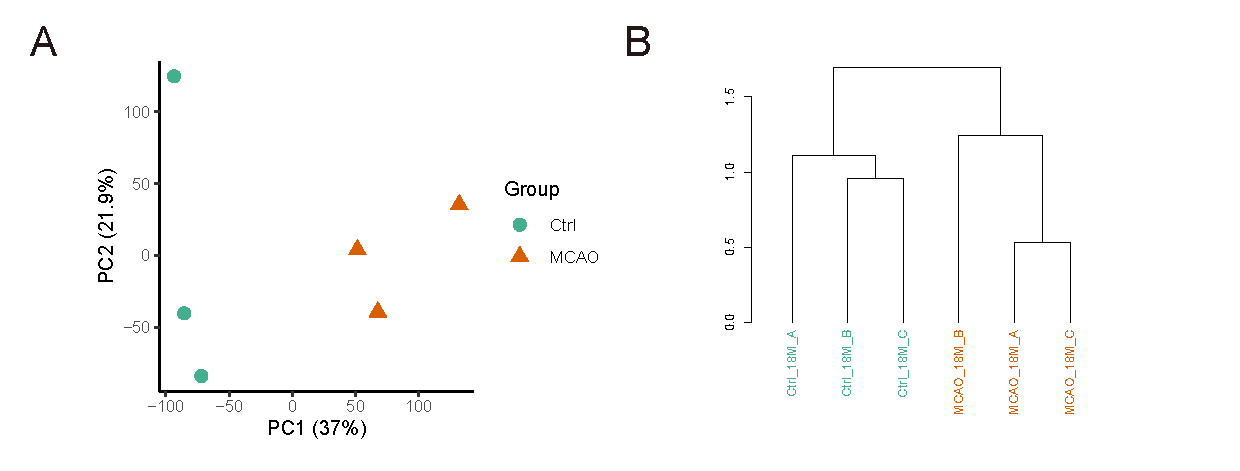
\includegraphics{./figure/Figure-2.pdf}

}

\caption{\label{fig-overview}\textbf{Data Overview}. \textbf{(A)} PCA
plot showing global similarity of genes expression in control and MCAO
samples. \textbf{(B)} Cluster Dendrogram based on Pearson distance
showing similarity among control and MCAO samples}

\end{figure}

\hypertarget{ischemic-aged-mice-have-a-large-number-of-upregulated-genes}{%
\subsection{Ischemic aged mice have a large number of upregulated
genes}\label{ischemic-aged-mice-have-a-large-number-of-upregulated-genes}}

As is shown in Figure~\ref{fig-differential}, after differential gene
expression analysis of genes between groups, 1,551 differential genes
were found in MAO mice compared to control mice
(\textbar log2FC\textbar\textgreater1; p-value \textless{} 0.05).
Moreover, the number of up-regulated genes was significantly higher than
that of down-regulated genes (up-regulated: log2FC\textgreater1,
down-regulated: log2FC\textless-1).

\begin{figure}[H]

{\centering \includegraphics{./figure/Figure-3.png}

}

\caption{\label{fig-differential}\textbf{Differential Gene Expression
Analysis}. \textbf{(A) } Differences in the number of up-regulated and
down-regulated genes between MAO and control mice (up-regulated:
log2FC\textgreater1, down-regulated: log2FC\textless-1). \textbf{(B) }
Volcano plots showing differential gene expression between MAO and
control mice. \textbf{(C) } Heatmap showing significantly differentially
expressed genes between MAO and control mice
(\textbar log2FC\textbar\textgreater1; p-value \textless0.05).}

\end{figure}

\hypertarget{ischemic-stroke-is-accompanied-with-increased-neuroinflammation-and-decreased-neurotransmitter-transport}{%
\subsection{Ischemic stroke is accompanied with increased
neuroinflammation and decreased neurotransmitter
transport}\label{ischemic-stroke-is-accompanied-with-increased-neuroinflammation-and-decreased-neurotransmitter-transport}}

Through Gene Ontology (GO) enrichment analysis of up-regulated genes and
down-regulated genes respectively, it was found that the GO Term of the
up-regulated genes is significantly enriched in inflammatory response
(such as regulation of immune effector process, leucocyte promotion,
mononuclear cell promotion, myeloid leucocyte activation), cell-cell
interactions (such as extraceller matrix organization, extraceller
structure organization, cell subtract adhesion), cell migration (such as
leukocyte migration, ameboidal type cell migration). On the other hand,
gene associated with neurotransmitter transport and potassium ion
channels et al., were downregulated (Figure~\ref{fig-go}).

\begin{figure}[H]

{\centering 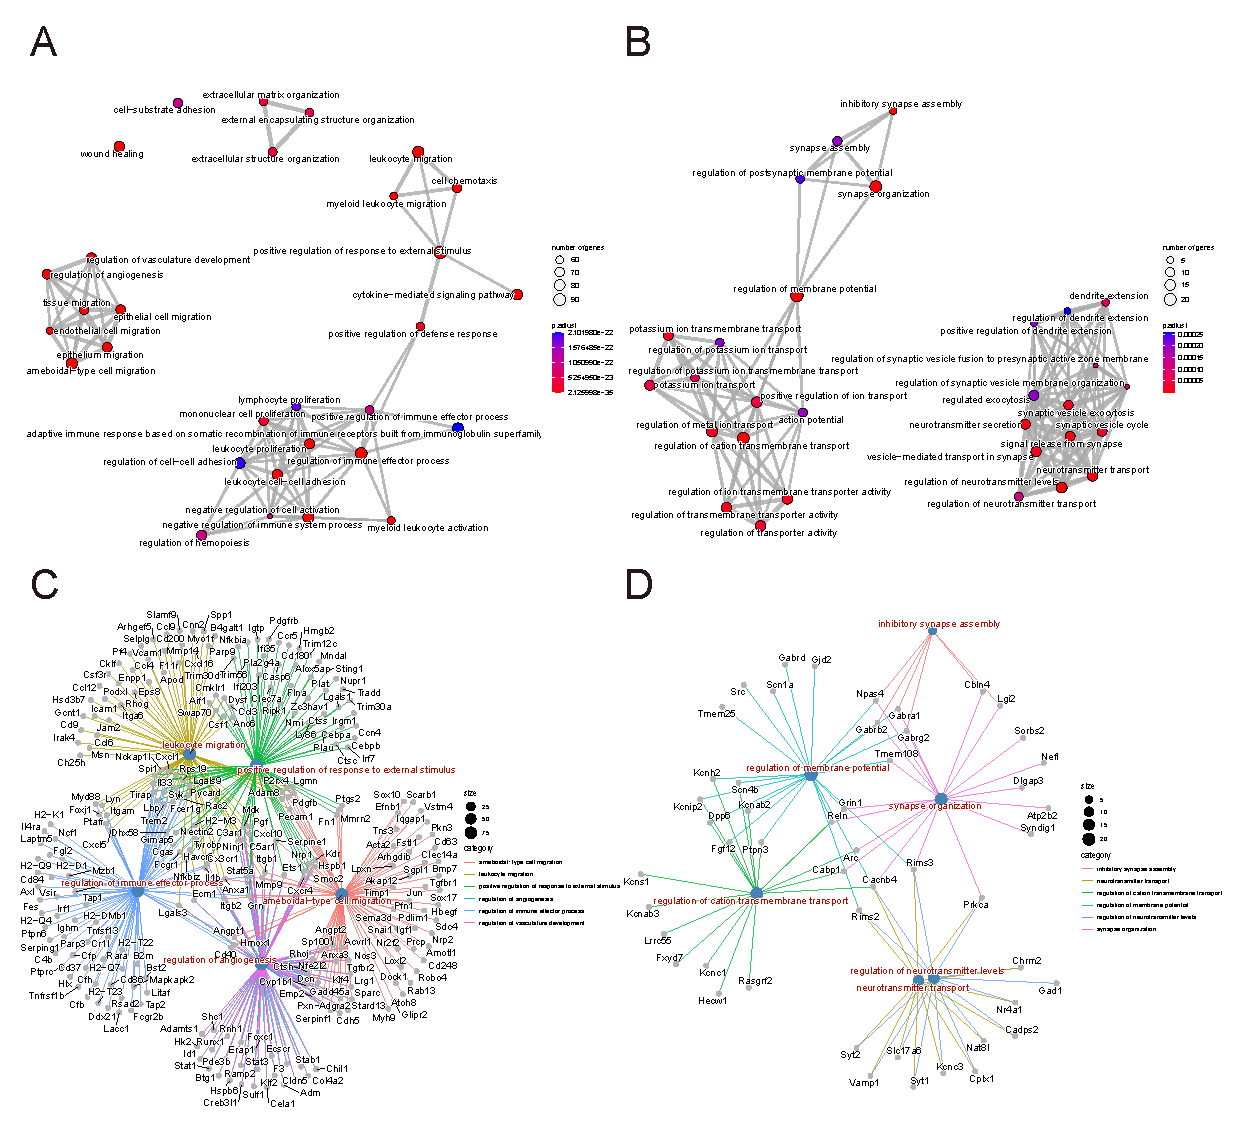
\includegraphics{./figure/Figure-4.pdf}

}

\caption{\label{fig-go}\textbf{Gene Ontology Enrichment Analysis}.
\textbf{(A)} Enrichment Map for enrichment result of up-regulated genes
in MAO mice. \textbf{(B)} Enrichment Map for enrichment result of
down-regulated genes in MAO mice. \textbf{(C)} Gene-Category Network for
enrichment result of up-regulated genes in MAO mice. Only the top 5
categories order by gene ratio are displayed. \textbf{(D)} Gene-Category
Network for enrichment result of down-regulated genes in MAO mice. Only
the top 5 categories order by gene ratio are displayed.}

\end{figure}

\hypertarget{discussion}{%
\section{Discussion}\label{discussion}}

In this study, transcriptome analysis was carried out in aged
post-stroke mice and normal mice. The results showed that the
up-regulated genes in stroke mice focused on inflammatory cascade and
peripheral leukocyte proliferation, which are the strongest producers of
reactive oxygen species (ROS) and matrix metallopeptidases (MMPs) and
promote neuronal injury and BBB disruption
\cite{allenOxidativeStressIts2009,streckerNeutrophilGranulocytesCerebral2017}.
The down-regulated genes may be related to neurotransmitter transport
and synaptic plasticity. Analysis results suggest that an increased
neuroinflammation and infiltration of circulating immune cells may be
one of the primary drivers for the exacerbated pathology in aged
post-stroke mice.

In conclusion, detailed insights into transcriptional response to stroke
described in this study may contribute to our understanding of the
interplay between stroke pathology and aging, and open avenues for the
future search for effective therapeutic approaches.

In addition, limited to time and server storage space, in terms of data,
only the aged samples were analyzed, whereas the young samples were
ignored. In terms of data analysis, Gene Set Enrichment Analysis (GSEA)
and Gene Co-expression Network Analysis (WGCNA) has not been conducted.
I hope there will be time to further study and improve the analysis
ability of bioinfomatics in the future.


\printbibliography[title=References]


\end{document}
